\section*{Question 2}
The unbalanced transportation problem was solved using the MODI Method, with all iterations shown in Figures~\ref{fig:q2_initial}--\ref{fig:q2_2}. The optimal solution can be seen in Figure~\ref{fig:q2_2}.

\begin{enumerate}[label=(\alph*)]
\item The optimal allocation is shown in Table~\ref{tab:q2}. As the demand exceeds supply, there is a shortage of 30m$^3$ for both locations B and C that must be fulfilled by external sources.

\begin{table}[htp]
\centering
\caption{Optimal Solution}\label{tab:q2}
\begin{tabular}{|l|l|}
	\hline
	Route & Allocation \\ \hline
	I-A   & 45         \\ \hline
	I-B   & 75         \\ \hline
	II-C  & 120        \\ \hline
	II-D  & 135        \\ \hline
\end{tabular}
\end{table}

\item The transportation cost corresponding to the solution obtained in part (a) is shown in Table~\ref{tab:q2_transport}.

\begin{table}[htp]
\centering
\caption{Transportation Cost}\label{tab:q2_transport}
\begin{tabular}{|lll|l|}
	\hline
	\multicolumn{1}{|l|}{Route} & \multicolumn{1}{l|}{Allocation} & Unit Cost & Total Cost \\ \hline
	\multicolumn{1}{|l|}{I-A}   & \multicolumn{1}{l|}{45}         & 9         & 405        \\ \hline
	\multicolumn{1}{|l|}{I-B}   & \multicolumn{1}{l|}{75}         & 10        & 750        \\ \hline
	\multicolumn{1}{|l|}{II-C}  & \multicolumn{1}{l|}{120}        & 6         & 720        \\ \hline
	\multicolumn{1}{|l|}{II-D}  & \multicolumn{1}{l|}{135}        & 3         & 405        \\ \hline
	\multicolumn{3}{|l|}{Total Cost}                                          & 2280       \\ \hline
\end{tabular}
\end{table}
\end{enumerate}


\clearpage

\begin{figure}[htp]
\centering
\caption{\label{fig:q2_initial}Initial Iteration}
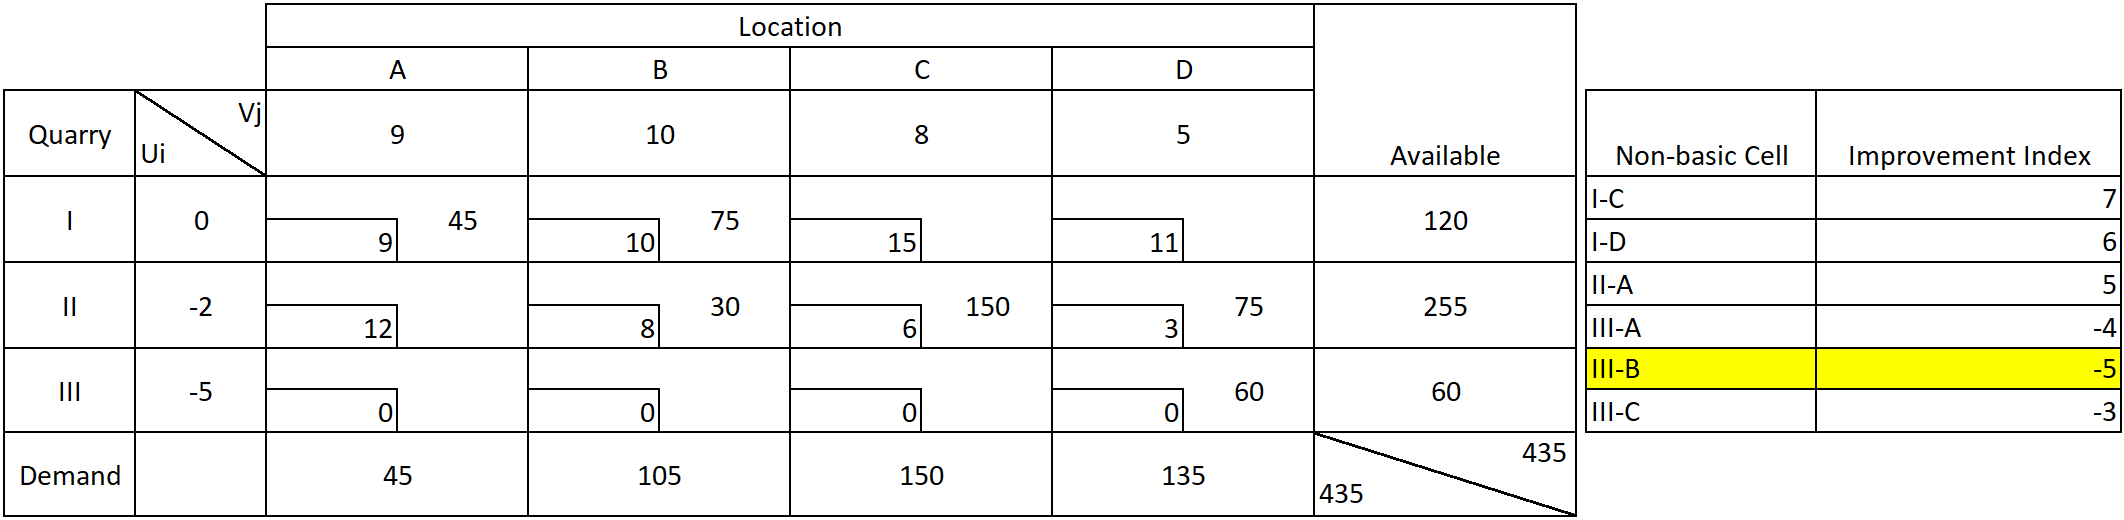
\includegraphics[width=\textwidth]{2_initial.png}
\end{figure}

\begin{figure}[htp]
\centering
\caption{\label{fig:q2_1}First Iteration}
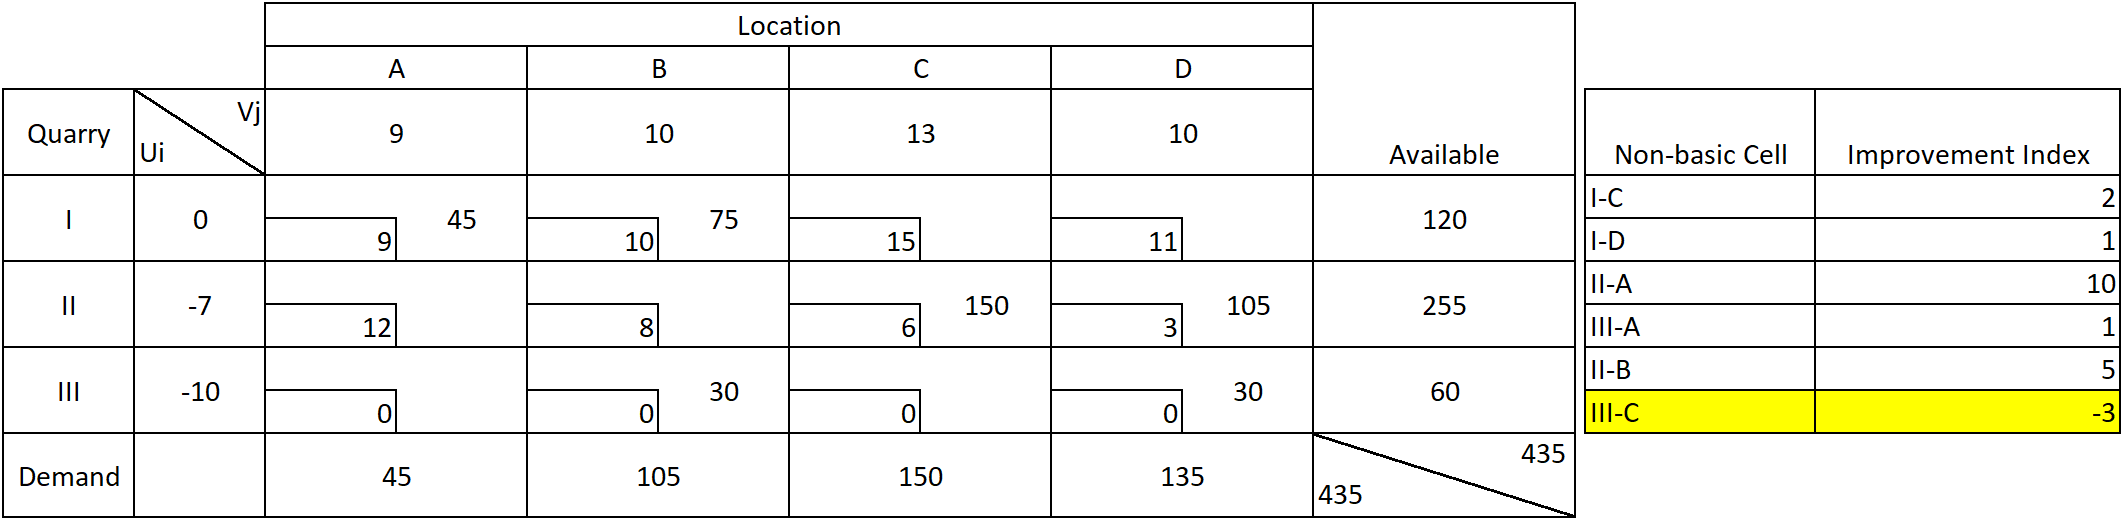
\includegraphics[width=\textwidth]{2_1.png}
\end{figure}

\begin{figure}[htp]
\centering
\caption{\label{fig:q2_2}Second Iteration}
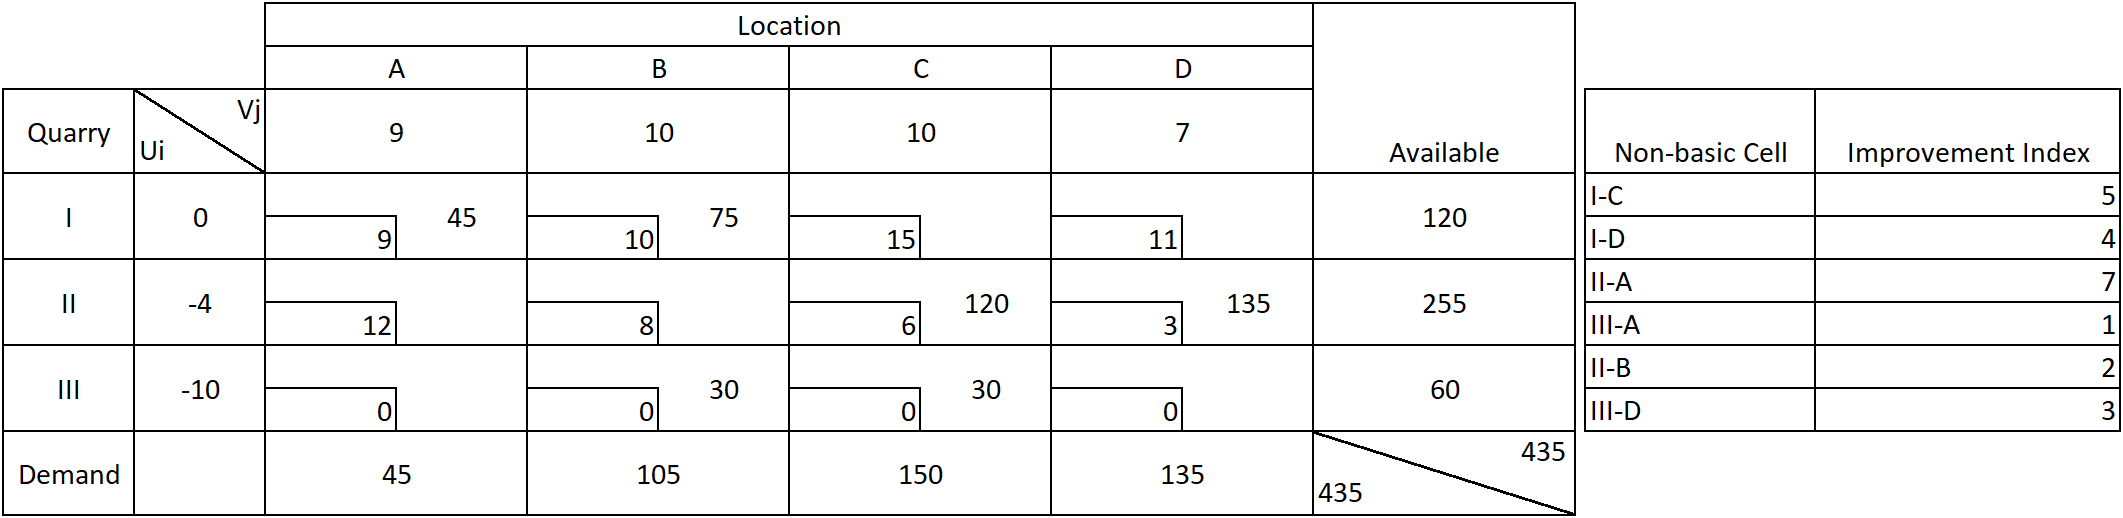
\includegraphics[width=\textwidth]{2_2.png}
\end{figure}